\documentclass[12pt]{article}
\usepackage[utf8]{inputenc}
\usepackage[english]{babel}
\usepackage{listings}
\usepackage{xcolor}
\usepackage{subcaption, hyperref}
\usepackage[braket, qm]{qcircuit} % Importa il pacchetto qcircuit
\hypersetup{
    colorlinks=false,
    linkbordercolor=white
}
\lstdefinestyle{python}{
    language=Python,
    basicstyle=\ttfamily\small,
    keywordstyle=\color{blue},
    stringstyle=\color{red},
    commentstyle=\color{green},
    morecomment=[s][\color{purple}]{/**}{*/},
    numberstyle=\tiny\color{gray},
    stepnumber=1,
    numbersep=10pt,
    frame=single,
    breaklines=true,
    postbreak=\mbox{\textcolor{red}{$\hookrightarrow$}\space},
    showspaces=false,
    showstringspaces=false
}
\lstset{style=python}

\usepackage{amsmath, amssymb, graphicx, algorithm, algpseudocode}

\linespread{1.6}
\title{Genetic algorithm for Quantum Support Vector Machines}
\author{Lorenzo Tasca}
\date{October 2024}

\begin{document}

%\maketitle
\tableofcontents

\newpage


\section{Introduction}

Quantum machine learning (QML) has recently gained attention as an emerging field of research in quantum information science, combining the principles of quantum computing and machine learning. \cite{biamonte2017} The main goal of QML is to leverage quantum phenomena like superposition, entanglement and interference to perform machine learning tasks. In contrast to traditional machine learning techniques, QML algorithms seem to offer potential benefits, as they can solve complex problems more efficiently and cost-effectively.

One of the most promising and most researched QML method at present is the Quantum Support Vector Machine (QSVM) \cite{havlicek2019}, an extension of the classical Support Vector Machine (SVM), a machine learning algorithm for classification and regression tasks. The classical SVM is one of the most used and popular models, that has been successfully applied to various fields, such as image recognition, text classification and bioinformatics. \cite{cristianini2000} However, as the complexity and the size of the dataset increases, classical SVMs are no longer able to perform efficiently. QSVM aims to overcome these limitations by leveraging the principles of quantum computing, constructing a quantum circuit that maps classical data into an exponentially large quantum Hilbert space, in this way hoping to achieve an exponential speedup. 

However, the design of such a circuit is often done manually, following for example standard practices and patterns, or some sort of rule of thumb. This approach may work for simple problems, but one quickly finds out that using hand-crafted circuits for non-trivial tasks leads to a bad performance of the model, as finding the correct ansatz by hand is too difficult. It is necessary to automate this process, i.e. we need an algorithm that designs a properly working quantum circuit from scratch. 

One way to attack this problem is by using a genetic algorithm. Genetic algorithms are meta-heuristic optimization algorithms inspired by the process of natural selection. In this work we develop a genetic algorithm that automatically designs, from first principles, the circuit to use in a QSVM classification, and we test it on various datasets. 

The algorithm was implemented exploiting the Python library Qiskit, for what regards the quantum device simulation, and scikit-learn, for the machine learning part. Qiskit is an open source Software Development Kit for working with quantum computers at the level of extended quantum circuits, operators, and primitives.

This work is organized as follows: in Chapter 2 we introduce how a classical SVM works, in particular we present the fundamental concept of kernelized SVM. In Chapter 3 we discuss the QSVM, we define what it is and see how it performs on some datasets. We will encounter the tedious problem of choosing the quantum embedding circuit. In Chapter 4 we introduce our genetic algorithm, and test its performance on several datasets. In Chapter 5 we draw conclusions and discuss possible future developments. 



\newpage
\section{Classical Support Vector Machine}

\subsection{General overview}

Machine learning (ML) is a subset of artificial intelligence, focused on developing algorithms that enable computers to learn from and make decisions based on data. A ML algorithm takes a set of $N$ samples of data, called \textit{dataset}, and automatically predicts properties of unknown data, without the need to give it explicit instructions. The dataset is often split into a \textit{training set}, on which the algorithm is trained on, and a \textit{test set}, utilized to evaluate the performance of the model. Data can be multidimensional, and each dimension is usually called \textit{feature}. 

ML algorithms can be classified in different categories: 
\begin{itemize}
    \item \textbf{Supervised learning}: each data point has a label that the model aims to predict. The label can be:
    \begin{itemize}
        \item Discrete, meaning the data can be separated into two or more classes and the goal is to use the training data to predict the labels for the test data. This task is called \textit{classification}. An example is identifying whether an image contains a dog or a cat, or diagnosing a medical condition as positive or negative based on patient records.
        \item Continuous, when each data is labelled by a continuous value, meaning the target variable can take on any value within a range and the model attempts to predict this continuous value. This is called \textit{regression}. For example, predicting the future price of a house based on its features is a regression problem.
    \end{itemize}
    \item \textbf{Unsupervised learning}: the dataset does not have labels, yet we would like to empirically determine something about the data. For example we may want to determine if the data can be represented as belonging to distinct groups (clustering).
\end{itemize}

In this work we will focus on the Support Vector Machine \cite{cristianini2000}, a supervised classification algorithm. 

Datasets vary from small simple dataset with 2 numerical features, up to large and complex datasets with thousands of numerical and categorical features. In our case, due to the limited computational power we possess, we will study only small 2D datasets.




\subsection{Support vector machine}

The Support Vector Machine (SVM) \cite{cristianini2000} is a binary classification algorithm, whose goal is to build the maximum margin separator between the two classes, that is, the separator that maximizes the distance of the closest point from each class. The standard SVM algorithm is a linear algorithm, so in particular it will try and build the separating margin as a hyperplane in a $d$-dimensional space (hence a $(d-1)$-dimensional plane), where $d$ is the number of features. The points that touch the margin, or that are on the wrong side of it, are called support vectors. The distance between the decision boundary and the support vectors is called margin. The algorithm will find the biggest possible margin. 

\subsubsection{Linear SVM}
Let's start assuming that the classes are linearly separable. We are provided with a dataset with $N$ $d$-dimensional instances $\{\mathbf{x}_i\}_{i=0,\cdots, N-1}$. The two classes will be labelled with $$y\in \{-1,1\}.$$ The margin will be the set of points 
\begin{equation}
    \{\mathbf{x}\in\mathbb{R}^d: w_0+\mathbf{w}^T\cdot \mathbf{x}=0\},
    \label{margin definition}
\end{equation}  
for appropriate parameters $w_0\in \mathbb{R}$ and $\mathbf{w}\in \mathbb{R}^d$, which define an hyperplane and must be found by the algorithm. Now we have to find $$\max_{w_0, \mathbf{w}}(m),$$ with the constraint 
\begin{equation}
    \frac{1}{||\mathbf{w}||}y_i(w_0+\mathbf{w}^T\cdot \mathbf{x_i})\geq m, \, \forall i=0,\cdots, N-1,
\end{equation}
that can be rewritten as 
\begin{equation}
    y_i(w_0+\mathbf{w}^T\cdot \mathbf{x_i})\geq m||\mathbf{w}||, \, \forall i=0,\cdots, N-1.
\end{equation}
The constraint prevents data points from falling into the margin. Rescaling $\mathbf{w}$ up to a multiplicative factor does not change the hyperplane it defines, so for convenience we can choose its norm such that 
\begin{equation}
    ||\mathbf{w}||=\frac{1}{m}.
\end{equation}
Therefore, the problem becomes minimizing
$$\frac{1}{2}||\mathbf{w}||, $$ with the constraint 
\begin{equation}
    y_i(w_0+\mathbf{w}^T\cdot \mathbf{x_i})\geq 1, \, \forall i=0,\cdots, N-1.
    \label{constraint hard margin}
\end{equation}
In the theory of convex optimization one can solve for the Lagrangian dual of this problem. We can introduce the dual variables $\alpha_i$ such that
\begin{equation}
    \mathbf{w}=\sum_{i=0}^{N-1}\alpha_iy_i\mathbf{x}_i.
    \label{alpha def}
\end{equation} 
One would obtain that the dual problem consists in maximizing, with respect to the weight vector $\mathbf{\alpha}\in\mathbb{R}^N$, the expression 
\begin{equation}
    f(\alpha_0,\cdots,\alpha_{N-1})=\sum_{i=0}^{N-1} \alpha_i-\frac{1}{2}\sum_{i=0}^{N-1}\sum_{j=0}^{N-1}\alpha_i\alpha_jy_iy_j(\mathbf{x}_i,\mathbf{x}_j),
    \label{dual problem SVM}
\end{equation}
with the constraint
\begin{equation}
    \alpha_i\geq 0,\,\,\,\,\,\,\,\,\,\forall i=0,\cdots, N-1,
\end{equation}
\begin{equation}
    \sum_{i=0}^{N-1}\alpha_iy_i=0.
\end{equation}
In eq. (\ref{dual problem SVM}) we indicated as $(\mathbf{x}_i,\mathbf{x}_j)$ the standard dot product of $\mathbb{R}^d$, explicitly
$$(\mathbf{x}_i,\mathbf{x}_j)=\mathbf{x}_i^T\cdot\mathbf{x}_j=\sum_{k=0}^{d-1}(\mathbf{x}_i)_k(\mathbf{x}_j)_k.$$
Eq. (\ref{dual problem SVM}) defines a quadratic programming
optimization problem, therefore the global maximum of $f$ can be efficiently found in the context of convex analysis. The parameter $w_0$ can be found by imposing that, for a support vector $$y_i(\mathbf{w}^T\mathbf{x}_i+w_0)=1,$$ that is, 
\begin{equation}
    w_0=\mathbf{w}^T\mathbf{x}_i-y_i.
\end{equation} 
Once the optimal $\alpha_i$ have been found, given a new instance $\mathbf{\tilde{x}}$, according to eq. (\ref{alpha def}) and eq. (\ref{margin definition}), we can predict its class calculating 
\begin{equation}
    \textup{sign}\left[\sum_{i=0}^{N-1}\alpha_iy_i(\mathbf{\tilde{x}}, \mathbf{x}_i)+w_0\right].
    \label{decision boundary svm}
\end{equation} 

What we just described is the so-called hard margin SVM \cite{cristianini2000}, because we did not allow points to fall inside the margin. One could relax this assumption, modifying the constraint in eq. (\ref{constraint hard margin}) into 
\begin{equation}
    y_i(w_0+\mathbf{w}^T\cdot \mathbf{x_i})\geq 1-\xi_i, \,\,\,\,\,\,\,\,\,\,\,\, \forall i=0,\cdots, N-1,
\end{equation}
where we introduced the slack variables $\xi_i$. We limit the softness of the margin by setting a positive constant $C$ such that 
$$ \xi\geq0,$$
\begin{equation}
    \sum_{i=0}^{N-1}\xi_i\leq C.
\end{equation}
This is called soft margin SVM. 

Scikit-learn \cite{pedregosa2011} provides a straightforward implementation of the SVM algorithm, which we can use to observe the algorithm in action through an example. We use a mock dataset with 2 features, so we can easily print the data, the decision boundary and the margin. 


\begin{lstlisting}
from sklearn.svm import SVC
from sklearn.datasets import make_blobs 

X,y = make_blobs(n_samples=200) #create mock dataset
svm = SVC(kernel='linear', C=1) #create svm
svm.fit(X, y) #fit the svm
\end{lstlisting}

The result of the fit is shown in Figure \ref{fig:classical svm mock}. We can observe how the algorithm built the largest possible margin. 

\begin{figure}[h!]
    \centering
    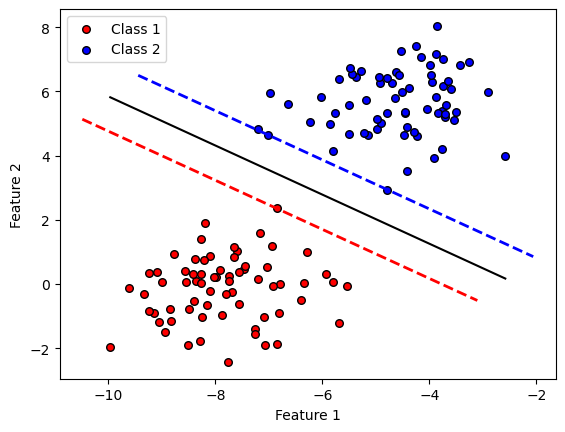
\includegraphics[width=0.8\textwidth]{images/classicalsvm.png}
    \caption{SVM decision boundary and margin border, fitted on a 2 feature mock dataset of 200 instances.}
    \label{fig:classical svm mock}
\end{figure}

\subsubsection{Kernel SVM}
We now need to address the issue of dealing with a highly non-linearly separable dataset. Let's consider as an example another mock dataset, shown in Figure \ref{fig:classical svm circles}. 
\begin{figure}[h!]
    \centering
    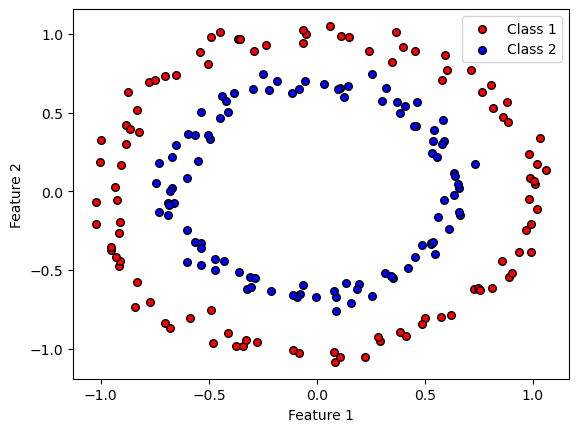
\includegraphics[width=0.8\textwidth]{images/circles.png}
    \caption{Higly non-linear 2 feature mock dataset with 200 instances.}
    \label{fig:classical svm circles}
\end{figure}
It is clear that in this case we cannot use the SVM algorithm in its basic form, not even with a soft margin. We must introduce the idea of kernelization. 
Let's introduce a function, called feature map, which projects the data in a higher dimensional space. That means a function
\begin{equation}
    \phi:\mathbb{R}^d\rightarrow\mathbb{R}^D,
\end{equation}
with $D>d$. The codomain of the feature map is called feature space. If we choose a suitable feature map we can hope to obtain a linearly separable dataset in the feature space. The choice of the feature map is completely arbitrary, as long as it is a bijective function. Therefore, in principle, each time we are given a dataset we must choose an appropriate feature map for this strategy to work. For our example let's consider the feature map
$$    \phi:\mathbb{R}^2\rightarrow\mathbb{R}^3,$$
\begin{equation}
    \begin{pmatrix}
        x_0\\
        x_1
        \end{pmatrix} \mapsto  
        \begin{pmatrix}
        x_0^2 \\
        x_1^2\\
        \sqrt{2}x_0x_1
        \end{pmatrix} .
\end{equation}
The data of Figure \ref{fig:classical svm circles} after the application of the feature map $\phi$ are represented in Figure \ref{fig:classical svm circle 3d}. 
\begin{figure}[h!]
    \centering
    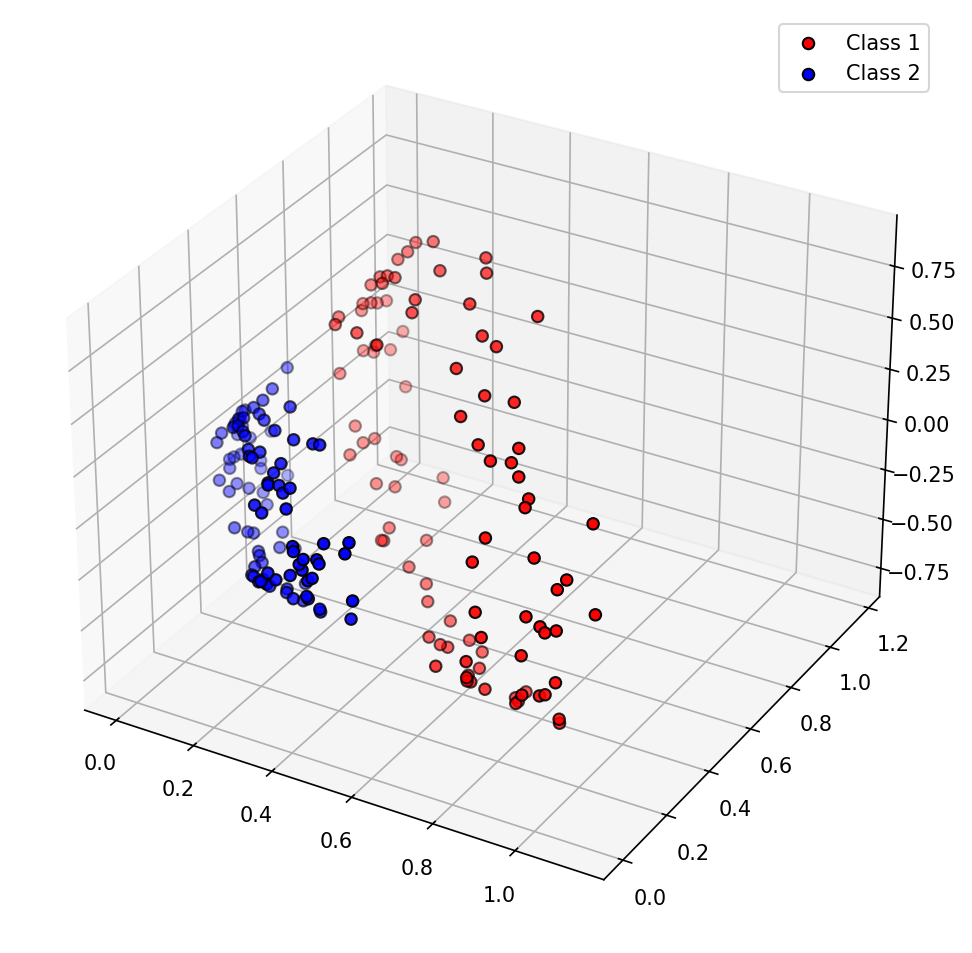
\includegraphics[width=0.8\textwidth]{images/circles3d.png}
    \caption{Highly non-linear mock dataset in the feature space after the application of the feature map $\phi$. We observe now that the dataset is linearly separable.}
    \label{fig:classical svm circle 3d}
\end{figure}
The dataset is now linearly separable in the feature space, so the strategy worked. We can now apply the SVM algorithm in this space. Consider the two central equations of the algorithm: equation (\ref{dual problem SVM}), which provides the expression to maximize in order to find the margin, and equation (\ref{decision boundary svm}), which gives the rule for predicting the class of a new instance. These two equations are now modified into 
\begin{equation}
    f(\alpha_0,\cdots,\alpha_{N-1})=\sum_{i=0}^{N-1} \alpha_i-\frac{1}{2}\sum_{i=0}^{N-1}\sum_{j=0}^{N-1}\alpha_i\alpha_jy_iy_j(\phi(\mathbf{x}_i,)\phi(\mathbf{x}_j)),
    \label{kernel max}
\end{equation}
\begin{equation}
    \textup{sign}\left[\sum_{i=0}^{N-1}\alpha_iy_i(\phi(\mathbf{\tilde{x}}), \phi(\mathbf{x}_i))+w_0\right].
    \label{kernel prodiction}
\end{equation}
A crucial observation is that in these two expressions only the scalar product of the feature map values appears. Therefore, we can conclude that the specific form of the feature map is not important, but rather the scalar product it produces. We can define the kernel $K$ as 
$$K:\mathbb{R}^d\times \mathbb{R}^d\rightarrow \mathbb{R},$$
\begin{equation}
    \mathbf{x}, \mathbf{y}\mapsto(\phi(\mathbf{x}), \phi(\mathbf{y})),
\end{equation}
 where $(\phi(\mathbf{x}), \phi(\mathbf{y}))=\phi(\mathbf{x})^T\cdot \phi(\mathbf{y})$ is the standard scalar product of $\mathbb{R}^D$. Eq. (\ref{kernel max}) and eq. (\ref{kernel prodiction}) now become 
 \begin{equation}
    f(\alpha_0,\cdots,\alpha_{N-1})=\sum_{i=0}^{N-1} \alpha_i-\frac{1}{2}\sum_{i=0}^{N-1}\sum_{j=0}^{N-1}\alpha_i\alpha_jy_iy_jK(\mathbf{x}_i,\mathbf{x}_j),
    \label{kernel max K}
\end{equation}
\begin{equation}
    \textup{sign}\left[\sum_{i=0}^{N-1}\alpha_iy_iK(\mathbf{\tilde{x}}, \mathbf{x}_i)+w_0\right].
    \label{kernel prodiction K}
\end{equation}
We see explicitly that the only quantity that matters is the kernel $K$. In our specific example the value of the kernel is 
\begin{equation}
    K(\mathbf{x}, \mathbf{y})= \begin{pmatrix}
        x_0^2 & x_1^2 & \sqrt{2}x_0x_1 \\
        \end{pmatrix}\cdot       \begin{pmatrix}
            y_0^2 \\
            y_1^2\\
            \sqrt{2}y_0y_1
            \end{pmatrix}=(\mathbf{x}^T\cdot\mathbf{y})^2.   
            \label{polykernel ex}   
\end{equation}
Therefore, once we are given a dataset it is sufficient for us to choose an appropriate kernel, and forget about the feature map. Once the kernel has been chosen the SVM can be trained using eq. (\ref{kernel max K}), and we can use it to predict a new class using eq. (\ref{kernel prodiction K}). There are some properties that the kernel must satisfy:
\begin{itemize}
    \item The kernel must be symmetric, that is $$\forall\, \mathbf{x},\mathbf{y}\in \mathbb{R}^d,\,K(\mathbf{x},\mathbf{y})=K(\mathbf{y},\mathbf{x}).$$
    \item The kernel must be positive definite, that is $$\forall\, \mathbf{x},\mathbf{y}\in \mathbb{R}^d,\,K(\mathbf{x},\mathbf{y})\geq 0.$$
\end{itemize}
Common choices of kernels are
\begin{itemize}
    \item Linear kernel: $$K(\mathbf{x},\mathbf{y})=\mathbf{x}^T\cdot\mathbf{y}.$$ This goes back to the standard SVM we used in Figure \ref{fig:classical svm mock}. It is suitable only for linearly separable (or close to, using soft margin) datasets.
    \item Polynomial kernel: $$K(\mathbf{x},\mathbf{y})=(\gamma\mathbf{x}^T\cdot\mathbf{y}+c)^\delta.$$ For $c=0$, $\gamma=1$ and $\delta=2$ we obtain the kernel of eq. (\ref{polykernel ex}). 
    \item Gaussian kernel: $$K(\mathbf{x},\mathbf{y})=\exp(-\gamma||\mathbf{x}-\mathbf{y}||).$$ This is also known as Radial Basis Function (RBF) kernel. 
    \item Sigmoid kernel: $$K(\mathbf{x},\mathbf{y})=\tanh(\mathbf{x}^T\cdot\mathbf{y}+c).$$
\end{itemize}
Scikit learn offers an easy way to easily implement all these common kernels. For example, the kernel in eq. (\ref{polykernel ex}) can be implemented as 
\begin{lstlisting}
    svm = SVC(kernel='poly', degree=2, gamma=1, coef0=0)
\end{lstlisting}\
One can also create a custom kernel, passing as an argument a callable function to be used to calculate the kernel. Fitting this SVC function to the non-linear dataset of Figure \ref{fig:classical svm circles} yields the result shown in Figure \ref{fig:classical svm circle decision boundary}. 
\begin{figure}[h!]
    \centering
    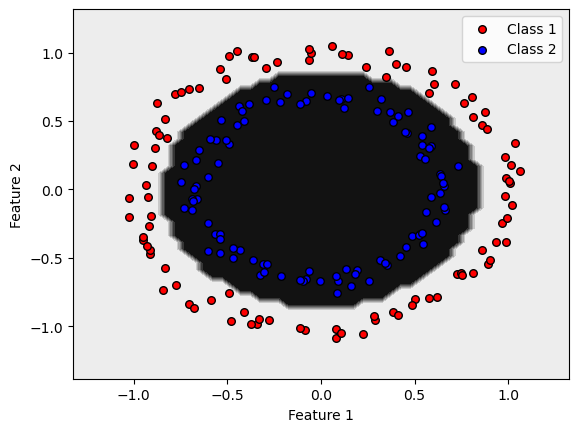
\includegraphics[width=0.8\textwidth]{images/circlesclassicaldecisionboundary.png}
    \caption{Highly non-linear mock dataset decision boundary, fitted with a SVM using kernel of eq. (\ref{polykernel ex}). The white and black areas are the two predicted classes. We observe how, using this kernel, we obtain a non-linear decision boundary.}
    \label{fig:classical svm circle decision boundary}
\end{figure}

\newpage \,
\newpage
\section{Quantum Support Vector Machine}
\subsection{General overview}
The concept of QSVM as we use today was first introduced in 2019, by Havlicek et al. \cite{primo} and, independently, by Schuld \cite{shuld}, that proposed and experimentally implemented the method on a superconducting processor. In 2021 Liu et al. established a rigorous quantum speedup for supervised classification using a general-purpose quantum learning algorithm that only requires classical access to data. Since then several interesting works have been published, but none faces the problem of how to build the quantum circuit to use to encode the classical data in the quantum device. This choice, we will see, is highly problematic, as already noted by Park et al. \cite{schifo}. In order to use the QSVM for real world applications it is mandatory to have a functioning way of finding the correct circuit to use.

\subsection{Quantum feature map and Quantum Kernels}
We anticipated how the classical SVM algorithm faces some important limitations when the feature space becomes large, as estimating kernel functions becomes computationally intensive. Quantum computing could enhance the algorithm's performance by providing access to exponentially large Hilbert feature spaces. The idea is to construct a feature map which maps classical data into a quantum state which lives in an exponentially large Hilbert feature space. Therefore, in this context a feature map is a function 
\begin{equation}
    \phi: \mathbb{R}^d \rightarrow \mathcal{H},
\end{equation}
$$\mathbf{x}\mapsto \phi(\mathbf{x})\equiv |\phi(\mathbf{x})\rangle.$$
In the framework of quantum computing $\mathcal{H}$ is a $n$-qubit Hilbert space, that is a space of the form
\begin{equation}
    \mathcal{H}=\bigotimes_{i=0}^{n-1} \mathcal{H}_{qubit},
\end{equation}
where $\mathcal{H}_{qubit}$ is the Hilbert space of a single qubit. The dimension of $\mathcal{H}$ is thus $2^n$. The feature map will be implemented by means of a parametrized quantum circuit. That means that it exists a unitary operator that depends on $d$ classical parameters $U(\mathbf{x})=U(x_0,\cdots, x_{d-1})$ such that 
\begin{equation}
    |\phi(\mathbf{x})\rangle=U(\mathbf{x})|0\rangle^{\otimes n}.
\end{equation}
This circuit is called \textit{quantum encoding circuit}, because it encodes classical data into a quantum state. The classical data is passed to the circuit as a parameter. We will later make examples of frequently used encoding circuits. 
Once we have the feature map, the kernel is constructed as 
\begin{equation}
    K(\mathbf{x}, \mathbf{y})=\left | \langle \phi(\mathbf{x})|\phi(\mathbf{y})\rangle \right |^2.
\end{equation}
Here $\langle\,\,, \,\rangle$ denotes the standard internal scalar product between vectors in $\mathcal{H}$. This definition clearly yields a kernel that satisfies the two kernel properties. How do we calculate the kernel in practice? Suppose we want to calculate the kernel $K(\mathbf{x}, \mathbf{y})$ and consider the following circuit. 

\begin{equation}
\Qcircuit @C=2em @R=2em {
   \lstick{|0\rangle} & \multigate{4}{U(\mathbf{x})} & \multigate{4}{U^\dagger(\mathbf{y})} & \meter\\
   \lstick{|0\rangle} & \ghost{U(\mathbf{x})}        & \ghost{U^\dagger(\mathbf{y})}        & \meter  \\
   \lstick{\vdots}    & \ghost{U(\mathbf{x})}        & \ghost{U^\dagger(\mathbf{y})}        & \vdots \\
   \lstick{|0\rangle} & \ghost{U(\mathbf{x})}        & \ghost{U^\dagger(\mathbf{y})}        & \meter  \\
   \lstick{|0\rangle} & \ghost{U(\mathbf{x})}        & \ghost{U^\dagger(\mathbf{y})}        & \meter  \\
} 
\label{circuit}
\end{equation}
\\
\noindent Suppose we run this circuit $R$ times, and we call $A$ the number of times that we measure the bit string $000\cdots 0$. We state that 
\begin{equation}
    \lim_{R\rightarrow +\infty}\frac{A}{R}=K(\mathbf{x}, \mathbf{y}).
    \label{frequency}
\end{equation}
The proof is straightforward. The left hand side of eq. (\ref{frequency}) is the probability of measuring $000\cdots 0$, which according to quantum mechanics can be calculated as 
$$
    |^{\otimes n}\textrm{$\langle$}0|U(\mathbf{x})U^\dagger(\mathbf{y})|0\rangle^{\otimes n}|^2=|^{\otimes n}\textrm{$\langle$}0|U^\dagger(\mathbf{y})U(\mathbf{x})|0\rangle^{\otimes n}|^2=$$$$=|\langle \phi(\mathbf{y})|\phi(\mathbf{x})\rangle|^2=K(\mathbf{x}, \mathbf{y}).
$$
\hfill $\square$

\noindent Therefore, to evaluate the kernel, it suffices to construct the quantum circuit (\ref{circuit}) and measure the frequency with which the string $000\cdots 00$ occurs. We have to perform this operation for each pair of instances, and construct the matrix 
\begin{equation}
    K_{ij}=K(\mathbf{x}_i, \mathbf{x}_j).
\end{equation}
This kernel matrix is then plugged into eq. (\ref{kernel max K}) to train a classical SVM. 

\subsection{Quantum encoding circuits}
Let's now discuss some possible choices of quantum encoding circuits:
\begin{itemize}
    \item Basis encoding: this can be applied if the instances live in a finite dimensional space, whose dimension is $2^n$, where $n$ is the number of qubits. If the dimension is smaller that $2^n$ we can still apply this encoding by using padding. The instances can be mapped into bit strings of length $n$ and the feature map corresponds to
    \begin{equation}
        \phi:\{0,1\}^n \rightarrow \mathcal{H},
    \end{equation}
    $$x=(x_0\cdots x_{n-1})\mapsto |x_0\rangle \otimes \cdots \otimes |x_{n-1}\rangle\equiv|x_0\cdots x_{n-1}\rangle=|x\rangle.$$ Here $|x\rangle$ is a state of the so called computational basis. For example, the bit string $01001$ is mapped to the quantum state $$|0\rangle \otimes |1\rangle \otimes |0\rangle \otimes |0\rangle \otimes |1\rangle=|01001\rangle.$$ The kernel that originates from this feature map is 
    \begin{equation}
        K(x,y)=|\langle x|y\rangle|^2=|\delta_{x,y}|^2=\delta_{x,y}
    \end{equation}
    since vectors in the computational basis are orthogonal, and $\delta$ is the Kronecker delta. 
    \item Amplitude encoding: this can be applied with instances that are normalized vectors, that is vectors of the form 
    \begin{equation}
        \mathbf{x}=(x_0, \cdots, x_{d-1})^T\in \mathbb{R}^d,
    \end{equation}
    such that $$\sum_{i=0}^{d-1}x_i^2=1.$$
    In this case, the encoding consists in mapping
    \begin{equation}
        \mathbf{x}=(x_0, \cdots, x_{d-1})^T \mapsto |\phi(\mathbf{x})\rangle=\sum_{i=0}^{d-1}x_i|i\rangle,
    \end{equation}
    where $|i\rangle$ is the i-th vector of the computational basis. The fact that $\mathbf{x}$ is normalized ensures that the feature vector is normalized as well, and therefore represents a physical state. The kernel generated by this feature map is 
    \begin{equation}
        K(x,y)=\left|\sum_{i,j}x_iy_j\langle i|j\rangle\right|^2=\left|\sum_{i,j}x_iy_j\delta_{i,j}\right|^2=(\mathbf{x}^T \cdot \mathbf{y})^2.
    \end{equation}
    As we can see we went back to a polynomial kernel. 
    \item By creating more copies of the feature vector in amplitude encoding, we can create higher order polynomial kernels. 
    \item Product encoding: in this case each feature of the input is encoded in the amplitudes of one separate qubit. For example, we can map
    \begin{equation}
        \mathbf{x}=(x_0, \cdots, x_{d-1})^T \mapsto  \begin{pmatrix}
            \cos x_0\\\sin x_0
           \end{pmatrix} \otimes \cdots \otimes \begin{pmatrix}
            \cos x_{d-1}\\\sin x_{d-1}
           \end{pmatrix},
    \end{equation}
    therefore the i-th qubit will be in the state 
    \begin{equation}
        \cos x_i|0\rangle +\sin x_i |1\rangle. 
    \end{equation}
    This generates the kernel 
    \begin{equation}
        K(x,y)=\prod_{i=0}^{d-1}\cos(x_i-y_i).
    \end{equation}
    \item ZZ feature map: The encoding maps discussed above are quantum maps that ultimately produce a kernel easily computable with classical tools, like a polynomial or cosine kernel. It is important now to discuss quantum encoding circuits which do not produce an easy classical kernel, otherwise there is no advantage in using quantum computing for this task if the kernel could always be easily calculated with classical tools. The hope is that by using a purely quantum kernel we obtain better performance than by using a classical kernel, in terms of classification or regression capability. Since general quantum circuits are not expected to be classically simulable, there are many choices one can make. One example is generated by the following circuit 

    \[
        \Qcircuit @C=3em @R=2em {
        \lstick{|0\rangle} & \gate{H} & \multigate{4}{\,\,\,\,\mathcal{U}(\mathbf{x})\,\,\,\,} & \qw \\
        \lstick{|0\rangle} & \gate{H} & \ghost{\,\,\,\,\mathcal{U}(\mathbf{x})\,\,\,\,}        & \qw \\
        \lstick{\vdots}    & \vdots   & \ghost{\,\,\,\,\mathcal{U}(\mathbf{x})\,\,\,\,}                    & \vdots \\
        \lstick{|0\rangle} & \gate{H} & \ghost{\,\,\,\,\mathcal{U}(\mathbf{x})\,\,\,\,}        & \qw \\
        \lstick{|0\rangle} & \gate{H} & \ghost{\,\,\,\,\mathcal{U}(\mathbf{x})\,\,\,\,}        & \qw \\
        }
    \]  
    \\
    where $H$ is the standard Hadamard gate and 
    \begin{equation}
        \mathcal{U}(\mathbf{x})=\exp\left[i\sum_{S\subseteq [n]}\phi_S(\mathbf{x})\prod_{i\in S}Z_i\right].
        \label{ZZ}
    \end{equation}
    Here $[n]=\{0,\cdots, n-1\}$, $Z_i$ is the third Pauli matrix acting on the $i$-th qubit, and $\phi_S(\mathbf{x})$ are arbitrary coefficients, which are the ones that actually encode the classical data. $S$ runs over all possible subsets of $[n]$, and can be thought of as an index that describes connectivities between different qubits or data points. We have $2^n$ possible choices of the coefficients. It is convenient to choose them in such a way that only the terms with $|S|\leq d$ contribute, in order to obtain a circuit that can be easily implemented on a quantum computer. This is done by asking that
    \begin{equation}
        \phi_S=0\,\,\,\,\,\textup{if}\,\,\,\,\,|S|>d.
    \end{equation}
    Let's focus on a simple case where $n=d=2$. There are two default choices for the coefficients in this case. The first one is to set 
    \begin{equation}
        \phi_{\{i\}}(\mathbf{x})=x_i,
        \label{coeff Z}
    \end{equation}
    \begin{equation}
        \phi_{\{i,j\}}(\mathbf{x})=0.
    \end{equation}
    The feature map becomes 
    \begin{equation}
        {U}(\mathbf{x})=e^{ix_0Z_0}\,e^{ix_1Z_1}H^{\otimes n}.
    \end{equation}
    This is called the \textit{Z feature map}. The corresponding circuit, decomposed in elementary quantum gates, is shown in Figure \ref{fig:Z}. 
    \begin{figure}[h!]
        \centering
        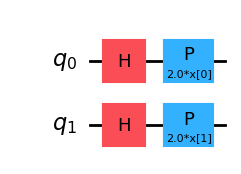
\includegraphics[height=100px]{images/Z.png}
        \caption{Z feature map, with 2 qubits and 2 features, decomposed in terms of elementary gates. The gate $P$ is defined as $P(\phi) = (1,0; 0, e^{i\phi})$, where $\phi$ is the parameter of the gate, and in our case can either be $2x_0$ or $2x_1$. We observe how the circuit is parametrized by the coefficients of eq. (\ref{coeff Z}).}
        \label{fig:Z}
    \end{figure}
    The other possible choice is  
    \begin{equation}
        \phi_{\{i\}}(\mathbf{x})=x_i,
        \label{coeff ZZ1}
    \end{equation}
    \begin{equation}
        \phi_{\{i,j\}}(\mathbf{x})=(\pi-x_i)(\pi-x_j).
        \label{coeff ZZ2}
    \end{equation}
    In this case the feature maps becomes 
    \begin{equation}
        {U}(\mathbf{x})=e^{i(\pi-x_0)(\pi-x_1)Z_0Z_1}\,e^{ix_0Z_0}\,e^{ix_1Z_1}H^{\otimes n}.
    \end{equation}
    This is called the \textit{ZZ feature map}, and it is an encoding circuit thought to be hard to simulate classically. It is shown in Figure \ref{fig:ZZ}. 
    \begin{figure}[h!]
        \centering
        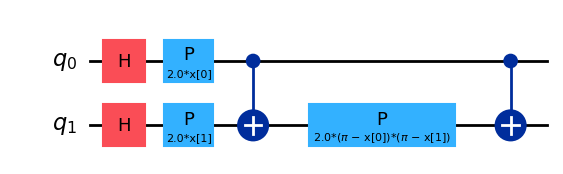
\includegraphics[height=100px]{images/ZZ.png}
        \caption{ZZ feature map, with 2 qubits and 2 features, decomposed in terms of elementary gates. The gate $P$ is defined as $P(\phi) = (1,0; 0, e^{i\phi})$, where $\phi$ is the parameter of the gate. The values that the parameter take are shown in the Figure, according to eq. (\ref{coeff ZZ1}) and (\ref{coeff ZZ2}).}
        \label{fig:ZZ}
    \end{figure}
    We will see how it behaves later on. Those two are standard choices, but there are many more circuits that can be built starting from the general structure of eq. (\ref{ZZ}), especially if we consider a greater number of qubits, and so we allow connectivities of three and more qubits. 
    \item Pauli feature map: Eq. (\ref{ZZ}) can be generalised to include not only Z gates, but all of the Pauli gates. We can have
    \begin{equation}
        \mathcal{U}(\mathbf{x})=\exp\left[i\sum_{S\subseteq [n]}\phi_S(\mathbf{x})\prod_{i\in S}P_i\right],
        \label{pauli}
    \end{equation}
    where $P\in\{1,X,Y,Z\}$. This allows us to generate not only interactions of the ZZ type, but also for example YY type or ZY type. An example with Y and ZY interactions is shown in Figure \ref{fig:Pauli}.
    \begin{figure}[h!]
        \centering
        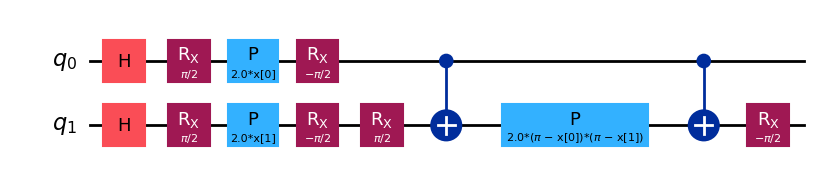
\includegraphics[width=\textwidth]{images/pauli.png}
        \caption{Pauli feature map, with 2 qubits and 2 features, decomposed in term of elementary gates, constructed with Y and YZ interactions.}
        \label{fig:Pauli}
    \end{figure}
    \item In general any parametrized quantum circuit can be used to encode classical data and create a quantum kernel. We will later use generic circuits and study what sort of datasets they separate.
\end{itemize}

\subsection{QSVM algorithm and Qiskit implementation}
To sum things up, the step of the Quantum Support Vector Machine (QSVM) algorithm are:
\begin{itemize}
    \item Prepare the classical data into two vectors $X$ and $y$, where $$X_i=\mathbf{x}_i \in \mathbb{R}^d,\, \,\,\,i=0,\cdots , N-1,$$ is the i-th $d$-dimensional instance, and $$y_i\in \{-1,1\},$$ indicates the class that this instance belongs to.  
    \item Choose a parametrized quantum circuit $U(\mathbf{x})$. The circuit accepts $d$ parameters, which are the features of the instance we are considering. One can choose a standard circuit like the ZZ feature map, or can create a custom circuit. We will extensively revisit the point of choosing the circuit later on.
    \item For each pair of instances $\mathbf{x}_i$, $\mathbf{x}_j$ we must evaluate the kernel matrix $$K_{ij}=K(\mathbf{x}_i,\mathbf{x}_j).$$ This is an $N\times N$ matrix, so for each pair we have build $U(\mathbf{x}_i)$ and $U^\dagger(\mathbf{x}_j)$, in order to construct the circuit     
    \begin{equation}
        \Qcircuit @C=2em @R=2em {
           \lstick{|0\rangle} & \multigate{4}{U(\mathbf{x}_i)} & \multigate{4}{U^\dagger(\mathbf{\mathbf{x}_j})} & \meter\\
           \lstick{|0\rangle} & \ghost{U(\mathbf{x}_i)}        & \ghost{U^\dagger(\mathbf{\mathbf{x}_j})}        & \meter  \\
           \lstick{\vdots}    & \ghost{U(\mathbf{x}_i)}        & \ghost{U^\dagger(\mathbf{\mathbf{x}_j})}        & \vdots \\
           \lstick{|0\rangle} & \ghost{U(\mathbf{x}_i)}        & \ghost{U^\dagger(\mathbf{\mathbf{x}_j})}        & \meter  \\
           \lstick{|0\rangle} & \ghost{U(\mathbf{x}_i)}        & \ghost{U^\dagger(\mathbf{\mathbf{x}_j})}        & \meter  \\
        } 
        \label{circuit item }
    \end{equation}
    and evaluate the matrix element 
    \begin{equation}
        K_{ij}=|^{\otimes n}\textrm{$\langle$}0|U(\mathbf{x}_iU^\dagger(\mathbf{x}_j)|0\rangle^{\otimes n}|^2.        
    \end{equation}
    As we saw this can be done, up to an error $R^{-1/2}$, by running the circuit (\ref{circuit item }) $R$ times and counting the number of times that we measure the string $000\cdots 0$.
    \item Once we have the kernel matrix we use classical optimization to maximize
    \begin{equation}
        f(\alpha_0,\cdots,\alpha_{N-1})=\sum_{i=0}^{N-1} \alpha_i-\frac{1}{2}\sum_{i=0}^{N-1}\sum_{j=0}^{N-1}\alpha_i\alpha_jy_iy_jK_{ij}.
        \label{loss function}
    \end{equation}
    Once we found the optimal $\alpha$ we have constructed the decision boundary.
    \item Given a new instance $\tilde{\mathbf{x}}$ we can, in the same way, calculate the kernel matrix element $$\tilde{K}_i=K(\mathbf{x}_i, \tilde{\mathbf{x}}),$$ and predict the class of $\tilde{\mathbf{x}}$ by applying \begin{equation}
        \tilde{y}=\textup{sign}\left[\sum_{i=0}^{N-1}\alpha_iy_i\tilde{K}_i+w_0\right].
    \end{equation}
\end{itemize}

Schematically we have 

\begin{algorithm}[H]
    \caption{Quantum Support Vector Machine (QSVM)}
    \begin{algorithmic}[1]
        \State \textbf{Input:} Data $\{(\mathbf{x}_i, y_i)\}_{i=0,\cdots,N-1}$, Quantum circuit $U(\mathbf{x})$
        \State \textbf{Parameters:} Measurement shots $R$
        
        \For{$i = 0 \textbf{ to } N-1$}
            \For{$j = 0 \textbf{ to } N-1$}
                \State \textbf{Prepare} $U(\mathbf{x}_i)$ and $U^\dagger(\mathbf{x}_j)$
                \State \textbf{Run} circuit $U(\mathbf{x}_i)U^\dagger(\mathbf{x}_j)$ $R$ times  
                \State \textbf{Measure} the frequency $f$ of $00\cdots 0$ 
                \State \textbf{Set} $f=K_{ij}$ 
            \EndFor
        \EndFor
        
        \State \textbf{Optimize} $\alpha$ to maximize
        \begin{equation*}
            f(\alpha) = \sum_{i=0}^{N-1} \alpha_i - \frac{1}{2} \sum_{i=0}^{N-1} \sum_{j=0}^{N-1} \alpha_i \alpha_j y_i y_j K_{ij}
        \end{equation*}
    
        \For{each new instance $\tilde{\mathbf{x}}$}
            \State \textbf{Compute} $\tilde{K}_i = K(\mathbf{x}_i, \tilde{\mathbf{x}})$
            \State \textbf{Predict} $\tilde{y} = \textup{sign}\left(\sum_{i=0}^{N-1} \alpha_i y_i \tilde{K}_i + w_0\right)$
        \EndFor
        
    \end{algorithmic}
    \end{algorithm}

This algorithm can be implemented in practice exploiting Qiskit to perform the circuit simulation and calculate the kernel, and subsequently using scikit-learn to perform the classical optimization once the kernel has been calculated. We can make an example, separating a mock dataset like in Figure \ref{fig:classical svm mock}, with a Pauli feature map. 

\begin{lstlisting}
    #create mock dataset
    X,y=make_blobs(n_samples=200) 
    #since the kernel involves rotation it is better to bring the data between 0 and pi
    X=MinMaxScaler(feature_range=(0,np.pi)).fit_transform(X) 
    #create quantum kernel
    kernel=FidelityQuantumKernel(feature_map=ZFeatureMap()) 
    #pass the kernel as a callable function 
    svm=SVC(kernel=kernel.evaluate) 
    #fit the svm
    svm.fit(X, y) 
\end{lstlisting}

The result of the fit is shown in Figure \ref{fig:qsvm}.
\begin{figure}[h!]
    \centering
    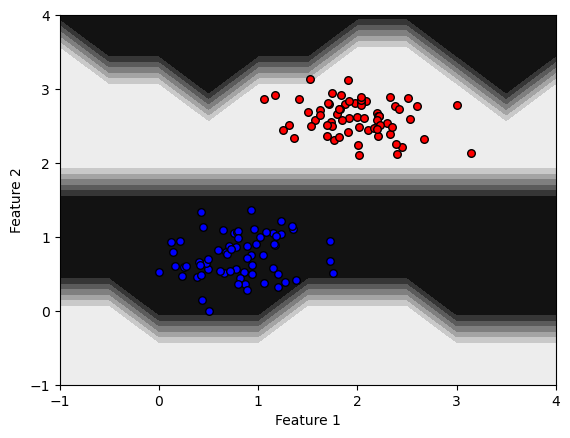
\includegraphics[width=0.8\textwidth]{images/qsvm.png}
    \caption{QSVM decision boundary with ZFeatureMap, fitted on a 2 feature mock dataset of 200 instances.}
    \label{fig:qsvm}
\end{figure}

\subsection{QSVM potential}
In order to study the potential of the QSVM algorithm we could try and observe the form of the decision boundary of an artificial dataset which is easily separable by a QSVM. If the decision boundary is "classically looking", that is similar to the one we observed when we studied the linear or polynomial kernel, then it would look like the QSVM algorithm may not provide advantage over the classical SVM. We hope instead to find a complex looking decision boundary, which is not separable by classical kernels. 

We use ZZFeatureMap, with $n=d=2$. Furthermore, we choose $f=Z_1Z_2$ and $V\in\textup{SU}(4)$. We assign $m(\mathbf{x})=+1$ when 
\begin{equation}
    \langle \phi(\mathbf{x}) |V^\dagger f V|\phi(\mathbf{x})\rangle >\Delta,
\end{equation} 
and $m(\mathbf{x})=-1$ when 
\begin{equation}
    \langle \phi(\mathbf{x}) |V^\dagger f V|\phi(\mathbf{x})\rangle <\Delta.
\end{equation} 
$\Delta$ controls how big is the gap between of the two classes. We show this dataset in Figure \ref{fig:adhoc}.
\begin{figure}[h!]
    \centering
    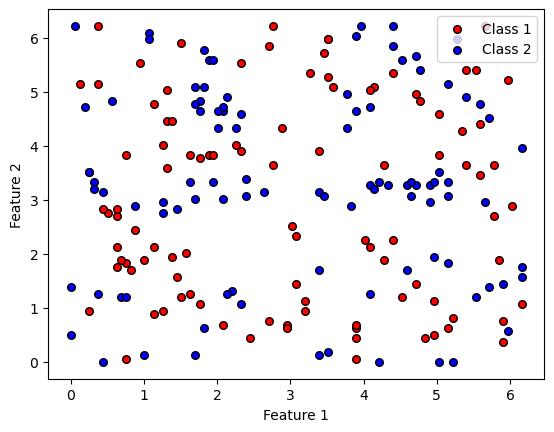
\includegraphics[width=0.8\textwidth]{images/adhoc.png}
    \caption{Artificial ad hoc dataset, generated with $\Delta=0.3$. This dataset, by construction, is easily separable by ZZFeatureMap.}
    \label{fig:adhoc}
\end{figure}
We observe how the dataset of Figure \ref{fig:adhoc} shows a very complicated pattern. Classical methods cannot hope to separate these two classes. In fact, if we divide the dataset into a training set and a test set, and apply the classical SVM algorithm, for example with the RBF kernel, we obtain an accuracy on the test set of 0.51, which is essentially like assigning the classes with a random coin toss. The result of the classical fit is shown in Figure \ref{fig:adhocrbf}, in which we observe how the correct decision boundary has not been found. 
\begin{figure}[h!]
    \centering
    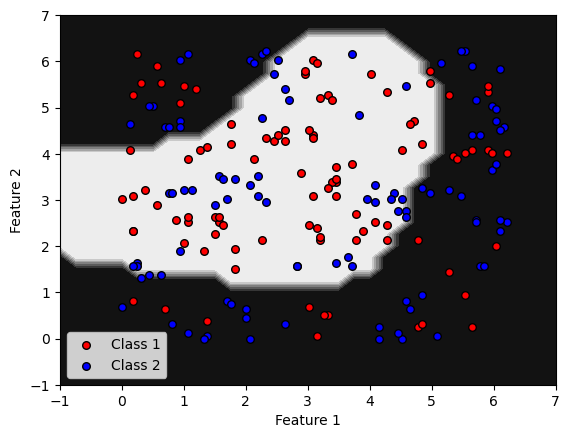
\includegraphics[width=0.8\textwidth]{images/adhocrbf.png}
    \caption{Result of the classical fit with RBF kernel on the artificial dataset. We observe how the SVM could not find the correct separation between the classes. }
    \label{fig:adhocrbf}
\end{figure}
In Figure \ref{fig:adhoczz} is shown instead the result of the fit with the QSVM with ZZFeatureMap, which yields an accuracy on the test set of 1.0, and a nice looking decision boundary. 
\begin{figure}[h!]
    \centering
    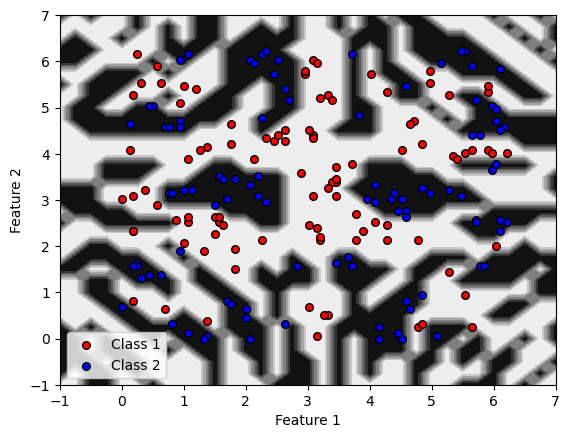
\includegraphics[width=0.8\textwidth]{images/adhoczz.png}
    \caption{Result of the quantum fit on the artificial dataset, with ZZFeatureMap. We observe how the QSVM found the correct separation between the classes.}
    \label{fig:adhoczz}
\end{figure}

Finding a dataset which is separable by quantum methods and not by classical methods leads us into thinking that the QSVM algorithm might outperform the SVM algorithm on datasets with complex patterns, which is the result we hoped to find. 

\subsection{Issues of QSVM}

In a QSVM algorithm the only choice the user has to make is the choice of the feature map, that is the choice of the quantum encoding circuit. It is easy to convince ourselves that this choice is crucial, and determines if the algorithm will be successful or not. In the classical case we also have to choose a kernel, but we found that this choice is much less delicate that in the quantum case. In fact, for example, the RBF kernel works very well for most applications. In the quantum case instead, we observed that the choice of the feature map is very tricky. If the wrong feature map is chosen, the QSVM performs very poorly even on very simple datasets, as we will now illustrate with some examples. Let's consider the dataset shown in Figure \ref{fig:classical svm circles}, which is simple enough to be expected to be separated without too many difficulties. We already saw of classical kernels separate this dataset very well. Let's try to apply some of the quantum kernels we discussed in the previous sections. 

We find that the results of the fits are not satisfying. The accuracy may not be too low in some cases, but the form of the decision boundary tells us that the algorithm did not find the correct pattern for the data. In some cases the algorithm may fail completely, like shown in Figure \ref{fig:failcircle}.
\begin{figure}[h!]
    \centering
    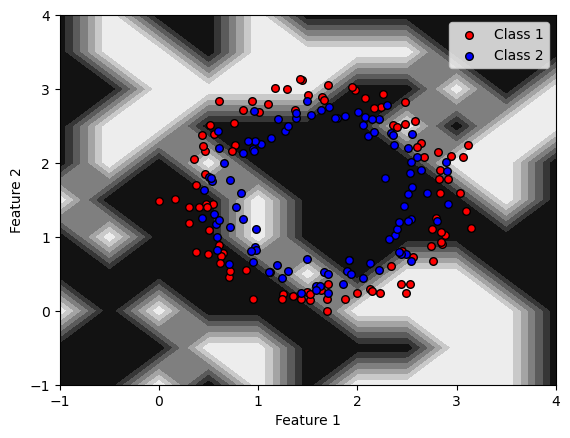
\includegraphics[width=0.8\textwidth]{images/failcircle.png}
    \caption{Circle dataset fitted with PauliFeatureMap leads to a very inaccurate decision boundary.}
    \label{fig:failcircle}
\end{figure}

It is clear at this point that the choice of the quantum encoding map is a very delicate part of the algorithm, and cannot be taken lightly. Choosing the feature map by trying the most common ones, as one may do with classical SVM, is not a safe method, as for a lot of datasets, even simple ones, the QSVM may fail. We need a more systematic way to choose the encoding, as the performance of the model is significantly influenced by this choice. We will discuss those methods in the next sections.

\subsection{Quantum kernel alignment}
\subsubsection{Circuit optimization}

In the previous sections, we discussed that the main challenge with the QSVM algorithm lies in selecting an appropriate feature map. This choice is difficult because there is no clear guidance in constructing the appropriate circuit, and the number of possible circuits for data encoding is potentially unlimited. Without guidance, it is problematic to select a circuit which works, since we saw how the choice of the feature map is very delicate. A first way to address this problem is the so-called Quantum Kernel Alignment (QKA). 

QKA is a hybrid quantum-classical approach, and consists in employing a parametrized quantum feature map $U(\mathbf{x}, \mathbf{\lambda})$, where we introduced $k$ parameters $\mathbf{\lambda}=(\lambda_0,\cdots, \lambda_{k-1})$ inside the feature map. The quantum circuit now has $d+k$ parameters, $d$ are passed through $\mathbf{x}$ and $k$ through $\mathbf{\lambda}$. However, the latter are fundamentally different from the former. The $\mathbf{x}$ parameters, as we saw, are the way the instance is passed to the circuit. The $\lambda$ parameters instead are just parameters which must be trained in order to find the best possible circuit. A parametrized feature map gives rise to a parametrized quantum kernel $$K_{i,j}(\mathbf{\lambda})=K_{\mathbf{\lambda}}(\mathbf{x}_i, \mathbf{x}_j),$$ and consequently to a parametrized objective function of the SVM
\begin{equation}
            f(\mathbf{\alpha}, \mathbf{\lambda})=\sum_{i=0}^{N-1} \alpha_i-\frac{1}{2}\sum_{i=0}^{N-1}\sum_{j=0}^{N-1}\alpha_i\alpha_jy_iy_jK_{ij}(\mathbf{\lambda}).
            \label{qka}
\end{equation}
Kernel alignment aims at minimizing the generalization error bound of SVM, and consists in solving the optimization problem
\begin{equation}
    \min_{\lambda}\max_{\alpha}f(\alpha, \lambda).
\end{equation} 
Here again $\alpha$ is the solution to the convex optimization problem of the SVM, while $\lambda$ is the variational parameter of the quantum circuit which must be trained. The optimization over $\alpha$ is performed as usual for the SVM. The optimization over $\lambda$ is performed using a Classical Simultaneous Stochastic Approximation (SPSA). The choice of SPSA lies in the fact that it needs less kernel evaluations compared to gradient descent methods, and it is more robust against noise, which is a serious issue of current real world quantum devices.    

QKA is a hybrid quantum-classical method, because the quantum circuit is utilized to evaluate the kernel when necessary, while all the other tasks such as optimizations are performed by classical algorithms. The fundamental steps of are:
\begin{itemize}
    \item Choose a parametrized quantum circuit $U(\mathbf{x}, \mathbf{\lambda})$, where $\lambda\in \mathbb{R}^k$.
    \item Choose an initial parameter $\lambda=\lambda_0$, and the maximum number of iterations $P$ of the SPSA algorithm.
    \item Generate random vector $\Delta \in \{-1,1\}^k$.
    \item Create two new parameters $\lambda_+$ and $\lambda_-$ such that $$\lambda_{\pm,i}=\lambda_i\pm c_i \Delta_i,$$ where $$c_i=\frac{c}{(i+1)^\gamma},$$ for chosen constants $c$ and $\gamma$. 
    \item Evaluate, using the QSVM standard approach on quantum device, the two kernels $$K_{\pm,ij}=K_{\lambda_{\pm}}(\mathbf{x}_i, \mathbf{x}_j).$$
    \item Find the solution $\alpha_{\pm}$ of the convex optimization problem in eq. (\ref{qka}), for the two kernels of the previous point, exploiting the standard SVM optimization.
    \item Perform two evaluations of the loss function to estimate its gradient with respect to $\lambda_k$: \begin{equation}
        g_k(\alpha_k, \lambda_k)=\frac{1}{2c_k\Delta_k}(f(\alpha_{+,k}, \lambda_{+,k})-f(\alpha_{-,k}, \lambda_{-,k})),
    \end{equation} where the loss function $f$ is given by eq. (\ref{qka}).
    \item Update $\lambda$ depending on the gradient $g_k(\alpha_k, \lambda_k)$ and the learning rate $a$. The update rule is \begin{equation}
        \lambda_{k+1}=\lambda_k-a_kg_k(a_k,\lambda_k).
    \end{equation}
    \item Repeat the procedure until the cost function has converged or the maximum number of iterations has been reached. 
    \item The final kernel is the optimal quantum kernel $K_{\lambda^*}(\underline{x}_i, \underline{x}_j).$
\end{itemize}

There are several possible choices for the insertion of the parameters in the quantum circuit. One common choice is to insert two parametrized rotations before the actual feature map, as shown in Figure \ref{fig:param rotation}. 
\begin{figure}[h!]
    \centering
    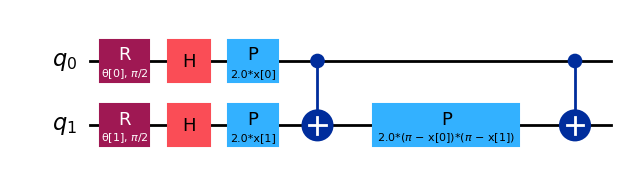
\includegraphics[width=\textwidth]{images/rotationsbeforeZZ.png}
    \caption{Parametrized quantum circuit, with two rotation inserted before a ZZFeatureMap.}
    \label{fig:param rotation}
\end{figure}
Another possible choice is to insert the parameters inside a ZZFeatureMap, and then apply the canonical ZZFeatureMap, as shown in Figure \ref{fig:ZZafterZZ}. The first one is parametrized by $\lambda$, while the second one by $\mathbf{x}$.
\begin{figure}[h!]
    \centering
    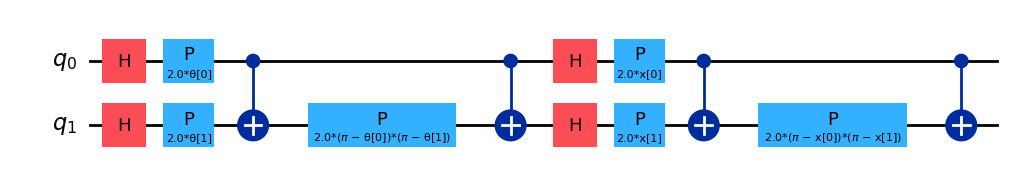
\includegraphics[width=\textwidth]{images/ZZafterZZ.png}
    \caption{Parametrized quantum circuit, with a ZZFeatureMap inserted before another ZZFeatureMap. The former has the parameters $\lambda$ for Quantum Kernel Alignment, while the latter has the parameters $\mathbf{x}$ in order to encode the classical instance.}
    \label{fig:ZZafterZZ}
\end{figure}

QKA can be implemented in Qiskit using the TrainableFidelityQuantumKernel class and the SPSA optimizer as following. 
\begin{lstlisting}
    kernel = TrainableFidelityQuantumKernel()
    cb_qkt = QKTCallback()
    spsa_opt = SPSA(maxiter=20, callback=cb_qkt.callback, learning_rate=0.05)
    loss = SVCLoss() #loss function for the SVM
    qkt = QuantumKernelTrainer(quantum_kernel=kernel, loss=loss, optimizer=spsa_opt)
    qka_results = qkt.fit(X_train, y_train) #optimize kernel
    optimized_kernel = qka_results.quantum_kernel
\end{lstlisting}
The final kernel is the optimized one, which can be used to train the QSVM and obtain the final result. 


\subsubsection{Performance}
We can evaluate the performance of the QKA-QSVM observing the behavior on the previously discussed datasets, in which the standard SVM algorithm performed badly. 
Let's consider for example the circular dataset of Figure \ref{fig:classical svm circles}. Let's use the feature map of Figure \ref{fig:param rotation}. 
The result is shown in Figure \ref{fig:qka}.
\begin{figure}[h!]
    \centering
    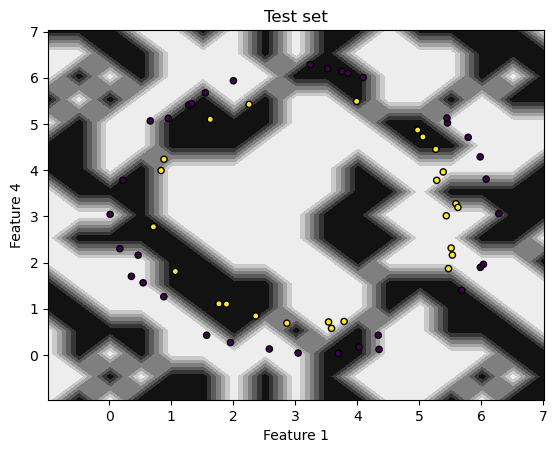
\includegraphics[width=0.8\textwidth]{images/qka.png}
    \caption{Result of the fit of circular dataset using QKA-QSVM. An accuracy of 50\% is achieved.}
    \label{fig:qka}
\end{figure}\\
The convergence of the SVC loss function and the final kernel is shown in Figure \ref{fig:loss function}. 
\begin{figure}[h!]
    \centering
    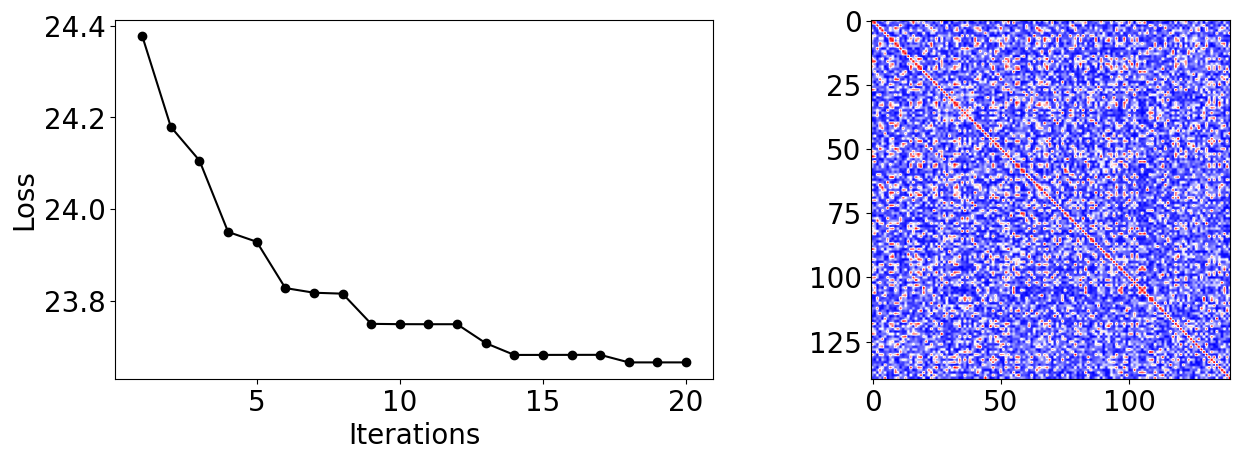
\includegraphics[width=\textwidth]{images/lossfunction.png}
    \caption{On the left convergence of the loss function during the QKA training. On the right the final trained kernel matrix.}
    \label{fig:loss function}
\end{figure}

We observe how even in this case the result is not satisfactory at all. The issue is that, even though now we have the freedom to insert parameters inside, it is still not clear how to choose the circuit or the parameters. This problem is not solved, consequently we are not capable of choosing a circuit which works for this particular dataset. We need to find a more advanced algorithm to choose the circuit.



\newpage
\section{Genetic algorithm}

A genetic algorithm can be used to choose the best feature map. We'll see how these types of algorithms can pick the right feature map based on first principles, without us having to decide the circuit's structure. Genetic algorithms have been previously used in the context of quantum computing, for example by Creevey et al. and Sünkel et al. We will apply this strategy for the QSVM case. 

\subsection{General introduction}

Genetic algorithms are optimization algorithms inspired by the process of natural selection, a key mechanism of biological evolution. The core concept is based on mimicking the biological evolution process, particularly principles like survival of the fittest, reproduction, mutation, and inheritance.

The primary components of the algorithm are the individuals, whose specific characteristics depend on the problem being addressed. Each individual is defined by a genotype and a phenotype. The genotype consists of a collection of genes, typically represented by numbers or character strings. The phenotype is a practical manifestation of the genotype, such as a quantum circuit or a neural network.

Individuals are organized into generations. The transition from one generation to the next occurs through crossover and mutation, mimicking the process of natural selection. A fitness function is defined to assess how well an individual performs in relation to the specific problem being addressed. The top-performing individuals in a generation, i.e., those with the highest fitness scores, can be passed directly to the next generation without undergoing crossover or mutation. This process is known as elitism.

Crossover emulates the crossing-over mechanism in meiosis. Two parent individuals from the current generation are selected with a probability proportional to their fitness, and two offspring are produced by combining the genotypes of the parents in a specific manner. Additionally, the offspring may undergo random gene mutations. The fitness of both offspring is then evaluated, with only the fittest being retained for the next generation. This way the generations all have the same number of individuals, to avoid an exponential growth of the dimension. This process is repeated multiple times to generate successive generations.

This process continues until either the maximum number of generations is reached or an individual achieves a predetermined target fitness level. Such individual is the result of the genetic algorithm. 

\subsection{Genetic algorithm for QSVM}





Let's now discuss how the above-mentioned concepts apply in the case of Quantum Support Vector Machine. The goal is to find the best possible feature map given a dataset. 

An individual is meant to represent a possible feature map choice. We define the genes of an individual in the form 
\begin{equation}
    [G, q_t, q_c, f],
\end{equation} 
where
\begin{itemize}
    \item $G$ is a gate chosen from a universal set of gates. For example, we can choose the set \begin{equation}
        \{X, \sqrt{X}, \textup{CNOT}, R_z\}.
    \end{equation}
    Here universal means that every possible gate can be generated using some combination of gates from this set. 
    $X, \sqrt{X}, \textup{CNOT}$ are fixed 1 and 2 qubit gates, whose matrix form is

\[
X = \begin{pmatrix}
0 & 1 \\
1 & 0
\end{pmatrix},
\]

\[
\sqrt{X} = \frac{1}{2} \begin{pmatrix}
1 + i & 1 - i \\
1 - i & 1 + i
\end{pmatrix},
\]

\[
\textup{CNOT} = \begin{pmatrix}
1 & 0 & 0 & 0 \\
0 & 1 & 0 & 0 \\
0 & 0 & 0 & 1 \\
0 & 0 & 1 & 0
\end{pmatrix}.
\]


On the other hand $R_z$ is a parametrized gate of the form

\[
R_z(\theta) = \begin{pmatrix}
e^{-i\theta/2} & 0 \\
0 & e^{i\theta/2}
\end{pmatrix}.
\]

Since the feature map is constituted by a parametrized quantum circuit $U(\mathbf{x})$, the parameters $\mathbf{x}$ will be inserted inside the $R_z$ type gates. 

\item $q_t$ is the target qubit to which the gate is applied, therefore it will be an integer number between $0$ and $n-1$, where $n$ is the number of qubits. 

\item $q_c$ is the control qubit, if it exists for that particular gate. If we use the gates set presented above only the $\textup{CNOT}$ gate has a control qubit, otherwise it is set to $\textup{None}$.

\item $f$ represents which feature to use as the gate parameter, if the gate accepts a parameter. In our example only the $R_z$ gate accepts one. In the other cases it is set to $\textup{None}$. Since we have $d$ features $(x_0, \cdots, x_{d-1})$, $f$ will be an integer between $0$ and $d-1$. 
\end{itemize}

The genotype will be a collection of genes of this form. The number of genes can vary, in particular it will represent the number of gates of the circuit. The phenotype associated to a genotype will be the corresponding parametrized quantum circuit. Let's make an example of this and consider $n=d=2$ and the genotype \\\ \{[$R_z$, 0, None, 0], [$R_z$, 1, None, 0], [CNOT, 1, 0, None], [$X$, 1, None, None]\}. \\\\ There are 4 genes, so the circuit must have first gate. If we look at the first gene we can conclude that the first gate is a $R_z$ with the first qubit as target. The control qubit is set to None since $R_z$ is a single qubit gate. The 0-th feature $x_0$ is used as the parameter of the circuit. Similar considerations hold for the others 3 gates. The circuit, i.e. the phenotype, is represented in Figure \ref{fig:fenotip}.
\begin{figure}[h!]
    \centering
    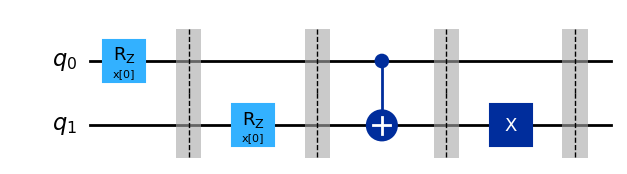
\includegraphics[width=0.8\textwidth]{images/fenotip.png}
    \caption{Example of the phenotype of an individual. The phenotype is a quantum circuit.}
    \label{fig:fenotip}
\end{figure}

We saw how parent individuals are passed to the child generation using crossover and mutations. Let's discuss how these operations are performed in the QSVM case. 

Crossover consists in cutting the circuit in half and pasting the two halves in two different children circuits. In formulas, assuming the number of genes $k$ to be even, starting from the parent genotype $$\{g^1_0, \cdots , g^1_{\frac{k}{2}-1}, g^1_{\frac{k}{2}}, \cdots, g^1_{k-1}\},$$$$\{g^2_0, \cdots , g^2_{\frac{k}{2}-1}, g^2_{\frac{k}{2}}, \cdots, g^2_{k-1}\},$$ we build the two children genotype $$\{g^1_0, \cdots , g^1_{\frac{k}{2}-1}, g^2_{\frac{k}{2}}, \cdots, g^2_{k-1}\},$$$$\{g^2_0, \cdots , g^2_{\frac{k}{2}-1}, g^1_{\frac{k}{2}}, \cdots, g^1_{k-1}\}.$$
In Figure \ref{fig:1par}-\ref{fig:2child} it is shown an example to illustrate what happens on the phenotype. 
\begin{figure}[h!]
    \centering
    \begin{minipage}{0.7\textwidth}
        \centering
        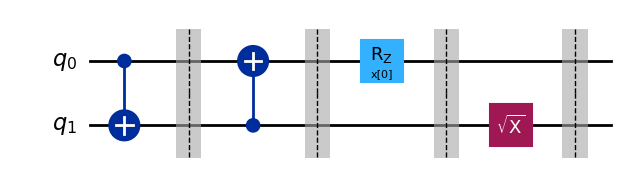
\includegraphics[width=\linewidth]{images/parent1.png}
        \caption{First parent phenotype.}
        \label{fig:1par}
    \end{minipage}
    \hfill
    \begin{minipage}{0.7\textwidth}
        \centering
        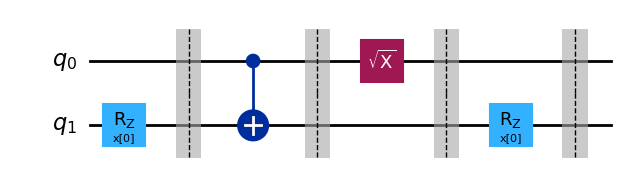
\includegraphics[width=\linewidth]{images/parent2.png}
        \caption{Second parent phenotype.}
        \label{fig:2par}
    \end{minipage}

    \vspace{0.5cm}

    \begin{minipage}{0.7\textwidth}
        \centering
        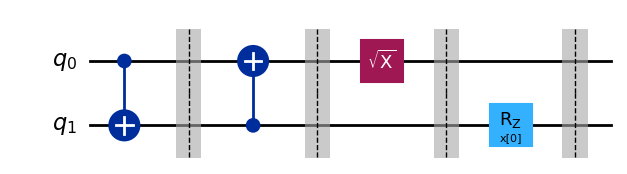
\includegraphics[width=\linewidth]{images/child1.png}
        \caption{First child phenotype.}
        \label{fig:1child}
    \end{minipage}
    \hfill
    \begin{minipage}{0.7\textwidth}
        \centering
        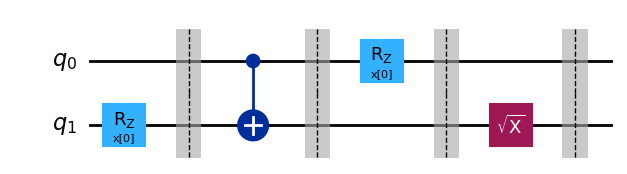
\includegraphics[width=\linewidth]{images/child2.png}
        \caption{Second child phenotype.}
        \label{fig:2child}
    \end{minipage}
\end{figure}

Mutation instead consists in a random mutation of the genes. That is every gene is mutated, with a probability $p$, into another randomly chosen. Another alternative way could be to mutate only one randomly chosen gene, with a probability of the mutation occurring greater than the former. An example is shown in Figure \ref{fig:mutated}-\ref{fig:nonmutated}.  
\begin{figure}[h!]
    \centering
    \begin{minipage}{0.7\textwidth}
        \centering
        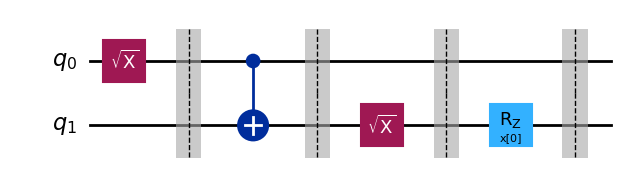
\includegraphics[width=\linewidth]{images/mutated.png}
        \caption{Starting non mutated individual.}
        \label{fig:mutated}
    \end{minipage}
    \hfill
    \begin{minipage}{0.7\textwidth}
        \centering
        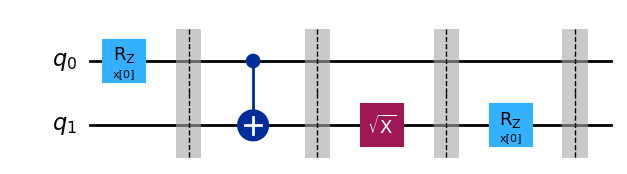
\includegraphics[width=\linewidth]{images/nonmutated.png}
        \caption{Mutated individual. The first gene is mutated from a $\sqrt{X}$ acting on the first qubit into an $R_z$ acting again on the first qubit. The other genes in this case were not mutated.}
        \label{fig:nonmutated}
    \end{minipage}
\end{figure}
This is a possible result of the mutation, of course being intrinsically random another mutation would produce a different result.  

The last concept we need to define in the QSVM case is the one of the fitness function. That is we need a quantitative way to assess how well an individual performs on the particular dataset we are considering. In machine learning there are several ways to evaluate the performance on a classification task. The simplest one is the accuracy on the test set, that is the ratio of correctly classified points and the total number of points. 
\begin{equation}
    \textup{accuracy}=\frac{\textup{correctly classified points}}{\textup{total number of points}}.
\end{equation}
For instance, we could use test set accuracy as the fitness of an individual. However, this approach would not sufficiently penalize poorly performing individuals, who are selected to generate offspring with a probability proportional to their fitness. If we use accuracy, an individual with a fitness of 0.5 has only half the probability of being chosen compared to one with a fitness close to 1. This is problematic because the former performs very poorly (its performance is comparable to randomly guessing the labels) whereas the latter correctly classifies almost every label. Moreover, individuals with a fitness below 0.5, which are not uncommon given the potential issues with the QSVM algorithm when an unsuitable feature map is selected, still have a non-negligible chance of being chosen. We would prefer these individuals to be heavily penalized, as their performance is even worse than random guessing. A possible way to achieve this is to use
\begin{equation}
    \textup{fitness}=\textup{accuracy}^6.
    \label{accuracy}
\end{equation}
The function is represented in Figure \ref{fig:fitness function}.
\begin{figure}[h!]
    \centering
    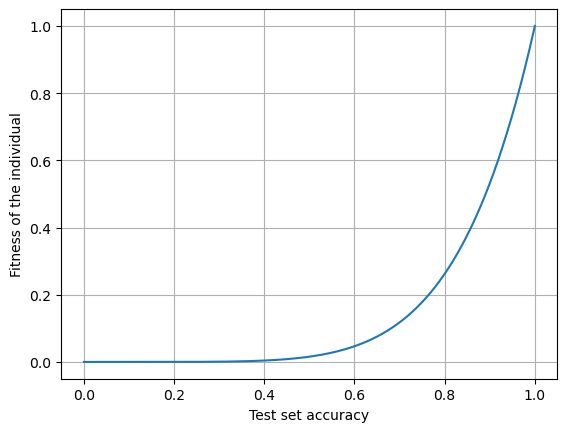
\includegraphics[width=0.8\textwidth]{images/sigmoid.png}
    \caption{Fitness of an individual as a function of its accuracy on the test set. This choice is made to properly penalize bad performing individuals.}
    \label{fig:fitness function}
\end{figure}
This choice strongly penalizes individuals with performance scores below 0.5, drastically reducing their chances of being selected for reproduction. Conversely, individuals with higher accuracy have significantly greater fitness, resulting in a much higher probability of being chosen to generate offspring.

Let us now provide a detailed explanation of how the algorithm functions. The initial inputs to the algorithm are as follows:
\begin{itemize} 
    \item A dataset, for which the objective is to discover a feature map that accurately classifies the data. This dataset will be split as usual into a training set and a test set. We will use the circular mock dataset of Figure \ref{fig:classical svm circles}, as we saw the difficulties of its classification without a genetic algorithm. The dataset automatically defines the number of features $d$.  
    \item The number $k$ of genes, that is the number of gates of the feature map. 
    \item The number $n$ of qubits that we want the circuit to have.
    \item The number of individuals $m$ that compose a generation.
    \item The percentage of individuals that automatically pass to the next generation through elitism. A typical value is $10\%$.
    \item The gate set to use to create the feature map. We will use $$\{X, \sqrt{X}, \textup{CNOT}, R_z\},$$ but other choices can be made, depending also on the type of physical architecture we plan on using for running the algorithm. For example Google Sycamore processor works by using the gates $$\{\sqrt{X}, \sqrt{Y},\sqrt{X+Y}, \textup{iSWAP}, \text{CZ}\},$$ so if we want to run the algorithm on that processor we could use this complete set of gates. 
    \item The probability $p$ of a mutation occurring on an individual. A standard value is 10\%.
    \item The target fitness we want to achieve. The algorithm will terminate if an individual reaches that target fitness. 
    \item The maximum number of generations we allow. If no individual achieves the target fitness the algorithm will terminate when the maximum number of generations is reached. 
\end{itemize}

The first step is to generate the first generation of individuals. This is done by randomly choosing $m$ circuits. Then the genetic algorithm begins, and works as follows:
\begin{itemize}
    \item The fitness of all the individuals is calculated.
    \item A fixed percentage of individuals, the one with the best fitnesses, are automatically passed to the next generation. 
    \item The remaining spots in the next generation are filled by children generated with crossover and mutations. For each spot two parents are chosen by randomly picking in the current generation, with a probability proportional to the fitness. Then two children are generated with crossover, and a random mutation is applied to each of them. The fitness of both children is evaluated and only the best one is kept and placed in the next generation. This procedure is repeated until the next generation is completely filled. Recall that all the generations have the same number of individual.
    \item This is repeated until an individual achieves the target fitness, or the total number of generations is reached.
    \item The best individual of the last generation is the result of the algorithm. In particular its phenotype is the best circuit that can be used in a QSVM to separate this particular dataset. 
\end{itemize}


\subsection{Results}

\subsubsection{Circle dataset}
We now execute the algorithm on the circular dataset shown in Figure \ref{fig:classical svm circles}. The genetic algorithm was implemented in Python, exploiting Qiskit to run the QSVM when necessary.

An important goal is to construct the smallest possible quantum circuit, minimizing both the number of gates and qubits. This is motivated by the technical limitations of current quantum devices, which struggle with larger, more complex circuits. Consequently, we begin with a simple circuit and will increase its depth or number of qubits if necessary.

For our experiment, we set a target fitness of 0.95, corresponding to an accuracy of 0.99, using eq. (\ref{accuracy}). We begin with a circuit with 2 qubits and 10 genes (gates), keeping the circuit compact.

The population size directly influences the efficiency of the algorithm. While larger populations provide more diversity and improve convergence, they significantly slow down the algorithm, particularly when using quantum simulators, like in our case. Since running a single QSVM instance already requires substantial time on a simulator, we opted for a reduced population size of 10 individuals. Although a standard starting point would be 100 individuals, we can begin with a small population and scale up if the results are unsatisfactory. We set a maximum number of 25 generations.

The initial parameters are shown in Table (\ref{tabella accettanza})
\begin{table}[h]
    \centering
    \begin{tabular}{||c c||} 
     \hline
     Parameter & Value  \\ [0.5ex] 
     \hline\hline
     Number of qubits & 2 \\ 
     Number of features & 2  \\
     Number of genes & 10  \\
     Target accuracy & 99\%  \\ 
     Maximum number of generation & 25  \\
     Individuals in a generation & 10  \\ 
     Individuals passed through elitism & 1 \\
     Probability of a mutation & 10\% \\  
     \hline
    \end{tabular}
    \caption{Parameters of the genetic algorithm}
    \label{tabella accettanza}
\end{table}

After 25 generations the algorithm reaches a fitness of 86\%. The final individual phenotype is represented in Figure (\ref{fig:final circuit}).
\begin{figure}[h!]
    \centering
    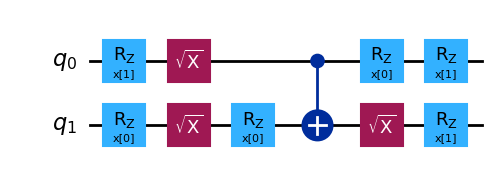
\includegraphics[width=0.8\textwidth]{images/finalcircuit.png}
    \caption{Final circuit of the genetic algorithm. This is the phenotype of the best individual of the last generation. This is the circuit with the best performance on this dataset that the genetic algorithm could find.}
    \label{fig:final circuit}
\end{figure}
This is the best-performing circuit identified by the genetic algorithm. Before exploring its potential, let's first assess whether the algorithm performed as expected. In Figure () we plot how the mean fitness of each generation evolves with the passing of generations. We observe an increase in the mean fitness, starting from a very low value in the first generation, which consists of randomly selected circuits, to a significantly higher value in the final generation. This confirms that the genetic algorithm is effectively improving the fitness of individuals through its internal crossover mechanics. If the mean fitness of the first generation was similar to that of the last, it would mean that the circuit was found by random chance, rendering the genetic algorithm useless. Instead, we clearly see how the algorithm consistently increases the fitness with each generation.
\begin{figure}[h!]
    \centering
    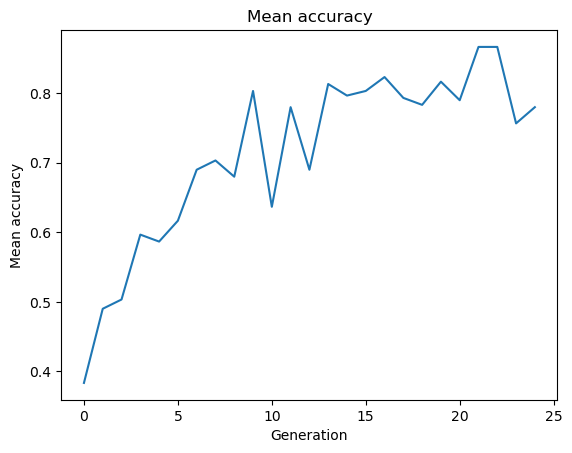
\includegraphics[width=0.8\textwidth]{images/meanaccuracy.png}
    \caption{Mean accuracy of each generation. We observe a consistent increase of the accuracy, ensuring that the genetic algorithm is improving the performance of the feature maps from generation to generation.}
    \label{fig:mean accuracy}
\end{figure}

To verify that the circuit in Figure \ref{fig:final circuit} can truly separate circle-like datasets, we tested its performance on a new artificial dataset. This dataset was generated using the same parameters as the one the circuit was trained on, but with new data points. It's essential to ensure that the circuit does not perform well only on the specific dataset it was trained with, but also on slightly varied datasets. The result of the fit is shown in Figure \ref{fig:awesome}, where we achieved 94\% accuracy. This indicates that the circuit is highly effective at separating circle-like datasets.
\begin{figure}[h!]
    \centering
    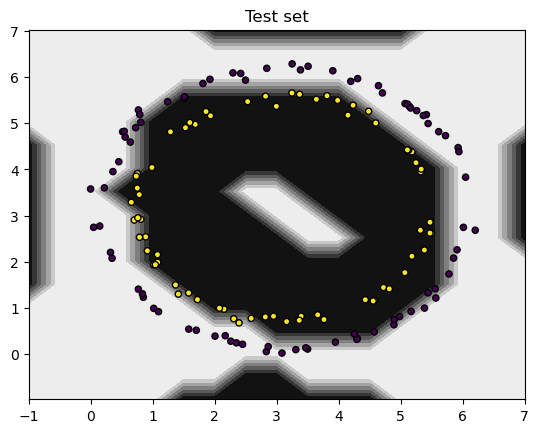
\includegraphics[width=0.8\textwidth]{images/awesomeresult.png}
    \caption{Final test of the resulting circuit of the genetic algorithm on a new dataset with respect the one it was trained on. The fact that the circuit is well performing on this dataset indicates that we actually found a circuit well performing on this sort of datasets.}
    \label{fig:awesome}
\end{figure}

To further demonstrate how the genetic algorithm improved the performance of the individuals, let's try the same task with an individual from the first generation. The result, shown in Figure \ref{fig:bad}, reveals poor performance, similar to the outcomes we observed when using standard feature map choices. So by just randomly picking circuits we are not able to construct well performing individuals. However, by evolving these individuals through crossover, the genetic algorithm is able to generate circuits with high accuracy for this type of dataset.
\begin{figure}[h!]
    \centering
    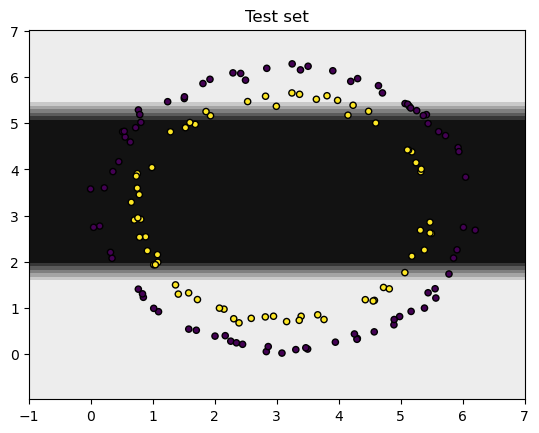
\includegraphics[width=0.8\textwidth]{images/badresult.png}
    \caption{Test of the performance of an individual from the first generation on the same dataset. We observe how its performance is very low, indicating that the first generation of individuals performs poorly as we expected.}
    \label{fig:bad}
\end{figure}

The fact that it performs well on this dataset is a strong indication of the potential of the final circuit we identified. However, it's natural to question how far this circuit can be pushed, as the dataset, while new, was still generated using the same parameters the genetic algorithm was trained on. What happens if we alter the shape by, for instance, adding noise or changing the radius of the two circles? Will the circuit still be able to classify correctly? Is the circuit able to classify all circle-like datasets? In Figure \ref{fig:noise} we used it to classify a different circle dataset, with noise added to the points. The classification reached a 91\% accuracy, indicating a good performance even on this dataset. We can answer affirmatively to the questions we asked.  
\begin{figure}[h!]
    \centering
    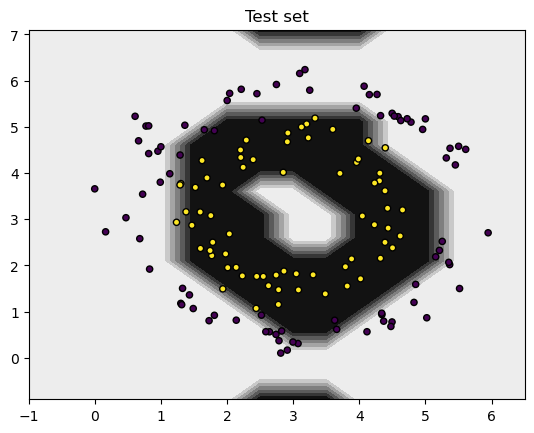
\includegraphics[width=0.8\textwidth]{images/noise.png}
    \caption{Test of the performance of the best individual on a new dataset with noise. The circuit is revealed to be robust against noise, correctly classifying 91\% of the point.}
    \label{fig:noise}
\end{figure}

\subsubsection{Moon dataset}

Let's now test the performance on another artificial dataset, the moon dataset. The algorithm conceptually works in the same way of the circle dataset, we utilized the same initial parameters as well, shown in Table (\ref{tabella accettanza}).

The resulting final circuit is shown in Figure \ref{fig:mooncircuit}, and its performance on the dataset in Figure \ref{fig:moonboh}, achieving an accuracy of 90\%. 
\begin{figure}[h!]
    \centering
    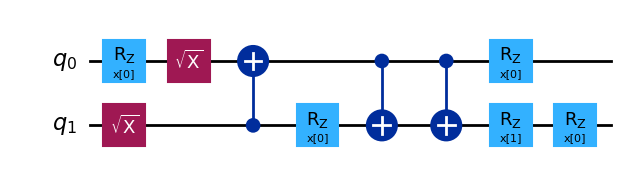
\includegraphics[width=0.8\textwidth]{images/mooncircuit.png}
    \caption{Final circuit of the genetic algorithm used on the moon dataset.}
    \label{fig:mooncircuit}
\end{figure}\begin{figure}[h!]
    \centering
    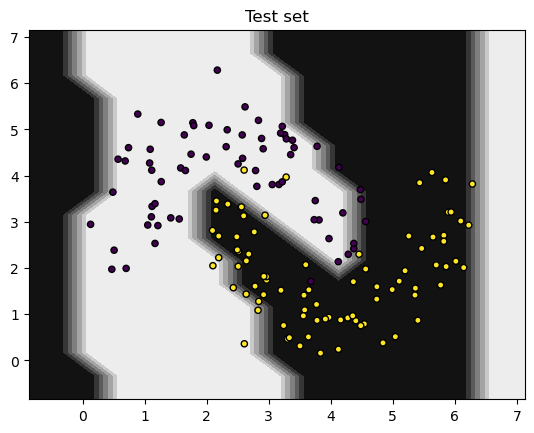
\includegraphics[width=0.8\textwidth]{images/moonboh.png}
    \caption{Performance of the final circuit on the moon dataset. Even in this case a good accuracy is achieved.}
    \label{fig:moonboh}
\end{figure}


\newpage 
\section{Conclusions}
The Quantum Support Vector Machine is an algorithm with great potential to outperform classical supervised classification models. Once fully implemented on a large scalable quantum device, we think it will successfully classify large datasets with many features and complicated patterns, that are intractable with classical methods. 

However we found it to be a very peaky algorithm in the choice of the quantum embedding circuit, so it is essential to use a proper algorithm to construct such a circuit, as using standard rule of thumb is often insufficient. The possibility we explored in this work is the one of a genetic algorithm. 

The algorithm showed great performance on simple 2D datasets, finding the optimal circuit that we were not able to find with other methods, opening the road to a broader application of genetic algorithms for QSVM, and in general in the field of Quantum Machine Learning. 

The goal now would be to further study the performance of the genetic algorithm we developed on larger multidimensional datasets, where the QSVM is expected to outperform classical algorithms. Conducting such tests on a quantum simulator, like Qiskit, would require significant computational resources, as simulating a quantum circuit on classical hardware is highly demanding. The ultimate goal therefore is to test the algorithm on a real scalable quantum device, its natural field of application. We are confident that it would show great performance, demonstrating its viability for real-world applications.


\newpage
\begin{thebibliography}{9}

    \bibitem{biamonte2017}
    Biamonte, J., Wittek, P., Pancotti, N., Rebentrost, P., Wiebe, N., \& Lloyd, S. (2017). \textit{Quantum machine learning}. Nature, 549(7671), 195-202. DOI:10.1038/nature23474.

    \bibitem{havlicek2019}
Havlíček, V., Córcoles, A.D., Temme, K., Harrow, A.W., Kandala, A., Chow, J.M., \& Gambetta, J.M. (2019). \textit{Supervised learning with quantum-enhanced feature spaces}. Nature, 567(7747), 209-212. DOI:10.1038/s41586-019-0980-2.

\bibitem{cristianini2000}
Cristianini, N., \& Shawe-Taylor, J. (2000). \textit{An Introduction to Support Vector Machines and Other Kernel-based Learning Methods}. Cambridge University Press.
    
\bibitem{pedregosa2011}
Pedregosa, F., Varoquaux, G., Gramfort, A., Michel, V., Thirion, B., \& Grisel, O. (2011). \textit{Scikit-learn: Machine Learning in Python}. Journal of Machine Learning Research, 12, 2825-2830.

\bibitem{sakurai}
Željko Ivezić, \emph{Statistics, Data Mining, and Machine Learning in Astronomy} (1994)

\bibitem{belkic}
Mitchell Melanie, \emph{An Introduction to Genetic Algorithms} (1999)

\bibitem{belkic}
A.E. Eiben, \emph{Introduction to Evolutionary Computing} (2003)

\bibitem{belkic}
Leo Sünkel, \emph{GA4QCO: Genetic Algorithm for Quantum Circuit
Optimization} (2023)

\bibitem{belkic}
Floyd M. Creevey, \emph{GASP: a genetic algorithm for state
preparation on quantum computers} (2023)

\bibitem{belkic}
Floyd M. Creevey, \emph{Kernel Alignment for Quantum Support Vector Machines Using Genetic
Algorithms} (2023)

\bibitem{belkic}
Thomas Hubregtsen, \emph{Training Quantum Embedding Kernels on Near-Term Quantum Computers} (2021)

\bibitem{belkic}
Jennifer R. Glick, \emph{Covariant quantum kernels for data with group structure} (2022)

\bibitem{belkic}
Maria Schuld, \emph{Supervised quantum machine learning models are kernel methods} (2021)

\bibitem{belkic}
Xiaojian Zhou, \emph{Quantum kernel estimation-based quantum support vector
regression} (2024)

\bibitem{belkic}
Seth Lloyd, \emph{Quantum embeddings for machine learning} (2022)

\bibitem{belkic}
Maria Schuld, \emph{Machine
Learning
with Quantum
Computers} (2021)

\bibitem{belkic}
N. Innan, \emph{Enhancing Quantum Support Vector Machines through
Variational Kernel Training} (2023)

\bibitem{shuld}
Maria Schuld, \emph{Quantum machine learning in feature Hilbert spaces} (2018)

\bibitem{primo}
Vojtech Havlicek, \emph{Supervised learning with quantum enhanced feature spaces} (2018)

\bibitem{belkic}
Jiaying Yang, \emph{Support Vector Machines on Noisy Intermediate
Scale Quantum Computers} (2019)

\bibitem{belkic}
Y. Liu, \emph{A rigorous and robust quantum speed-up in supervised machine learning} (2020)


\bibitem{belkic}
Patrick Rebentrost, \emph{Quantum support vector machine for big data classification} (2014)

\bibitem{schifo}
Jae-Eun Park, \emph{Practical application improvement to Quantum SVM} (2020)







\end{thebibliography}










\end{document}